\chapter{Positioning} \label{ch:positioning}

This chapter is about recognizing the position of a device either in absolute coordinates or relative to an earlier fix. We will cover absolute positioning where we derive our position by measuring our distance to fixed beacons in our environment. Relative positioning is on the other hand about estimating our position relative to a previous absolute position. Finally we will discuss hybrid positioning which is a combination of measuring our position and estimating movement until a new absolute measurement is made.

\section{Absolute positioning}
\section{Relative positioning}

A relative position is a position that is relative to something absolute. A technique called dead reckoning is very useful in situations where one have to move away from a absolute position, therefore will not be able to get another for a while. Such as in a network game or outside hiking with no Global Positioning System (GPS). To use dead reckoning you need to keep track of things that can help you navigate, such as:

\begin{itemize}
\item Direction of travel.
\item Pace.
\item Time of walking.
\item Landmarks.
\end{itemize}

When our hiking trip starts, we know we are at a absolute position, that is our base camp, and we want to reach the destination as shown in figure \ref{fig:deadrecdrawing}. We use our pace, compass and the landmarks to navigate to the destination.

\begin{figure}[H]
	\centering
	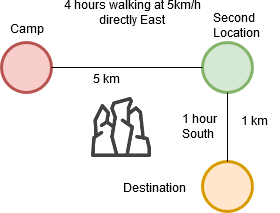
\includegraphics[width=0.4\linewidth]{positioning/positioning/deadRecDrawing}
	\caption{A hiking trip with navigation using dead reckoning.}
	\label{fig:deadrecdrawing}
\end{figure}

But dead reckoning suffers from errors that are cumulative, for example, if the first part of the trip had ended up being 8 kilometers instead of 5 then even if the second part goes according to plan, you are still going to end up in the wrong place. A way to solve this problem is to find your absolute location with bearings from time to time as that will reset the drift in regard to possible errors.

\section{Dead recking in network games}

Dead recking is not only used at sea or to navigate at land, but also in distributed virtual environments. When people across the planet play network games, they are sometimes located very far from each other, geographically. Pantel and Wolf\footnote{\cite{Pantel2002}} explores different dead reckoning schemes in various games such as sports and action games. They measured eight prediction schemes: Four predictions of positions, three predictions of input and one with no prediction. As shown in Figure \ref{fig:wolfpeperimage} Prediction 1 which predicts the position by assuming a constant velocity yields the best result.

\begin{figure}[H]
	\centering
	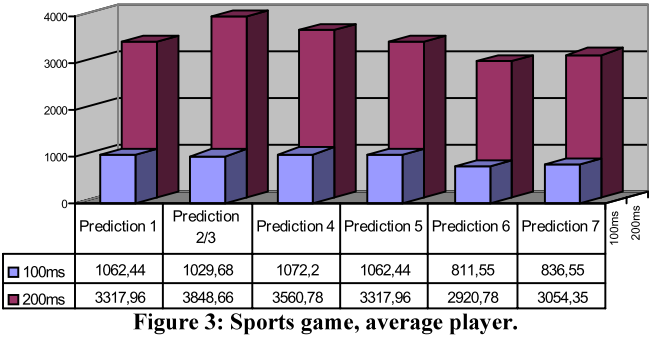
\includegraphics[width=0.5\linewidth]{positioning/positioning/wolfpeperImage}
	\caption{Prediction 1 was best in a sports game}
	\label{fig:wolfpeperimage}
\end{figure}

The article concludes that the different schemes tested upon were useful for network games, but could not reduce the latency directly, the impact, on the game, could be reduced however.
\section{Hybrid positioning}

The absolute positioning method is quit accurate but still it suffers from noise. On the other hand relative position has a lot uncertainty, because of the physical interference. By combing these two positioning methods we can get more precise location based on sensor measurements from absolute and prediction from the relative positions. This combination is called hybrid positioning. One of the methods achieving hybrid position is with Kalman filter, which will be described below.

\subsection{Kalman filter}

The Kalman filter was made by Rudolf E. Kalman. It was developed for Apollo mission to the moon, to track the location of the space shuttle. This method is still used, because it dos not require a lot of processing power and memory space. The reasoning is that the method dos not need to save any data apart the model of movement and and previews position.

The process of the filter is as follow:
\begin{enumerate}
	\item Predict the position form previews position and movement of the model
	\item Correct the position with the measured data
	\item Repeat step 1 and 2
\end{enumerate}

Fidure\ref{fig:KalmanfilterRotation} shows it visually.

\begin{figure}[H]
	\centering
	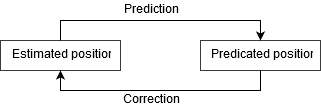
\includegraphics[width=0.4\linewidth]{positioning/positioning/KalmanFilterProcess}
	\caption{Kalmans filter principal}
	\label{fig:KalmanfilterRotation}
\end{figure}

In the Figure\ref{fig:Kalmanfilter} is displayed two case how the filter works. First one is when time(T-1) and time(T). In this case the filter goes closer to the measurement Gaussian, because it is more reliable.The hybrid position probability is higher then absolute and relative positioning this is because the absolute and relative position Gaussian's are multiplied together. The second case is in the period (T) and (T+1) in this case the measurements has a lot more noise in them. Then the estimation is moving further from the measurement Gaussian, because of the lower probability. 

\begin{figure}[H]
	\centering
	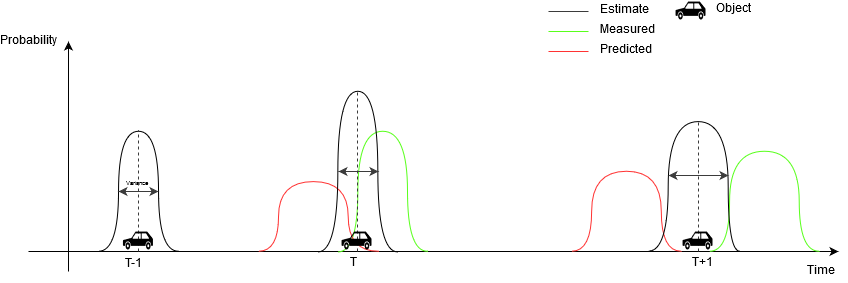
\includegraphics[width=0.7\linewidth]{positioning/positioning/DiagramKalman}
	\caption{Kalmans filter example}
	\label{fig:Kalmanfilter}
\end{figure}

%\section{Hybrid positioning and Kalman filter}
%The absolute positioning method is quit accurate but still suffers from noise. On the other hand relative positioning has a lot of uncertainty, because of the physical interference. By combing these two positioning methods we can get more precise location based on sensor measurements from absolute and prediction from the relative positions. This combination is called hybrid positioning. One of the methods achieving hybrid position is with Kalman filter.
%The Kalman filter was made by Rudolf E. Kalman and developed for the Apollo 11 mission\footnote{\cite{Grewal2010}} to the moon to track the location of the space shuttle. This method is still used because it does not require a lot of processing power or memory space. The reasoning is that the method does not need to save any data apart from the model of movement and the previous position. The filter predicts a position based on the model and previous positions. After the prediction, the real position is being measured and the filter corrects its prediction by multiplying both Gaussian distributions thus producing a more precise prediction of position.
%In figure \ref{fig:Kalmanfilter} we see how the filter is working. There are two cases in it. First one is when time is (T-1) and (T). In this first case we can see that the filter goes closer to the measured distribution, because it is more reliable. Also from the graph we can see the power of hybrid position: The probability is estimating the position correct is higher than absolute and relative positioning. The second case is when time is (T) and (T+1). In this case the measurements contain a lot more noise. Then the estimation is moving further from the measured distribution because of the lower probability.
%The Kalman filter was made by Rudolf E. Kalman. It was developed for Apollo mission to the moon, to track the location of the space shuttle. This method is still used, because it dos not require a lot of processing power and memory space. The reasoning is that the method dos not need to save any data apart the model of movement and and previews position.
%In the Figure\ref{fig:Kalmanfilter} is displayed two case how the filter works. First one is when time(T-1) and time(T). In this case the filter goes closer to the measurement Gaussian, because it is more reliable.The hybrid position probability is higher then absolute and relative positioning this is because the absolute and relative position Gaussian's are multiplied together. The second case is in the period (T) and (T+1) in this case the measurements has a lot more noise in them. Then the estimation is moving further from the measurement Gaussian, because of the lower probability.
